\newpage
\section{Analysis and Design}

\subsection{Analysis}

\subsubsection{Business process modelling}

Processes are modelled as activity diagrams. Swimlanes separate the actor from the system.

\begin{figure}[H]
\centering
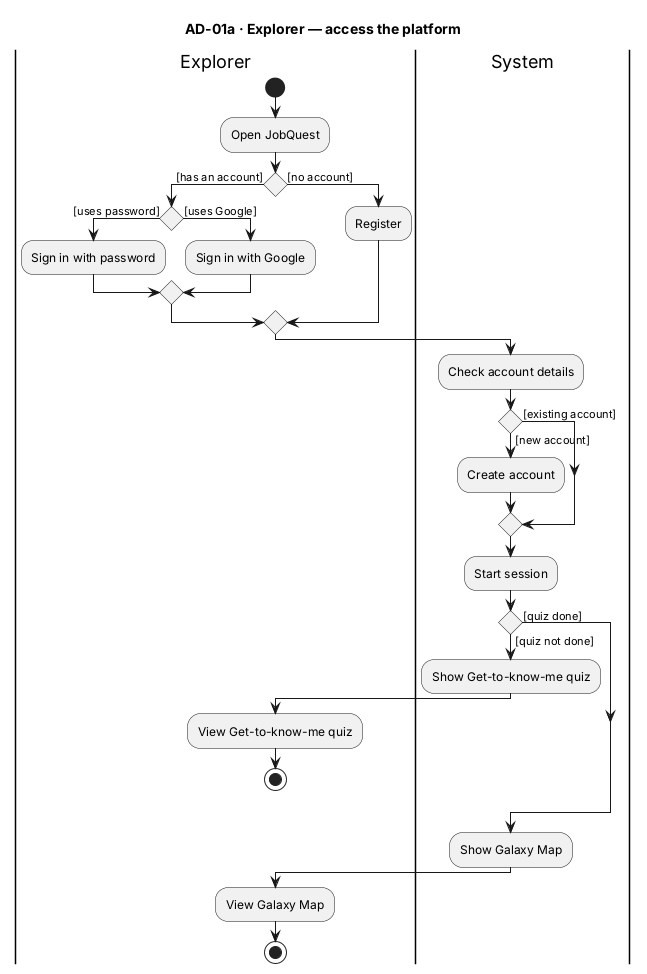
\includegraphics[width=0.59\textwidth,height=0.85\textheight,keepaspectratio]{figures/AD-01a_Explorer_AccessPlatform.png}
\caption{Explorer: access the platform (AD-01a)}
\end{figure}

\subsubsection{Use case modelling}

Use case descriptions follow, grouped by actor.

\begin{usecase}{UC-E01}{Register account}
\ucrow{Dependencies}{%
  \ucitem{FR-01 \textit{Register, sign in with a password or Google, and recover the account}}
  \ucitem{NFR-17 \textit{Passwords hashed, traffic encrypted}}}
\ucrow{Description}{The system shall behave as described in the following use case when \textit{a visitor without an account creates one to start exploring}.}
\ucrow{Precondition}{\textit{The visitor has opened JobQuest and is not signed in.}}
\ucsteps{Ordinary Sequence}
\ucstep{1}{Actor \textit{visitor opens JobQuest}.}
\ucstep{2}{The system \textit{checks access and shows the sign-in screen}.}
\ucstep{3}{Actor \textit{visitor chooses to register and provides the account details}.}
\ucstep{4}{The system \textit{creates the account and starts a session}.}
\ucrow{Postcondition}{\textit{The account exists and the explorer is signed in.}}
\ucsteps{Alternative Sequence}
\ucstep{3}{Actor \textit{visitor chooses to sign in with Google}. The sequence \textit{continues at step 4}.}
\ucsteps{Exceptions}
\ucstep{3}{If \textit{the visitor already has an account}, then this use case \textit{is cancelled}.}
\ucrow{Comments}{\textit{Passwords are stored as salted hashes (NFR-17).}}
\end{usecase}

\subsection{Design}

\subsubsection{Sitemap Design}

A sitemap has one box per screen; a solid arrow is navigation the user chooses and a dashed arrow is a screen the system leads to after an action.

\begin{landscape}
\begin{figure}[H]
\centering
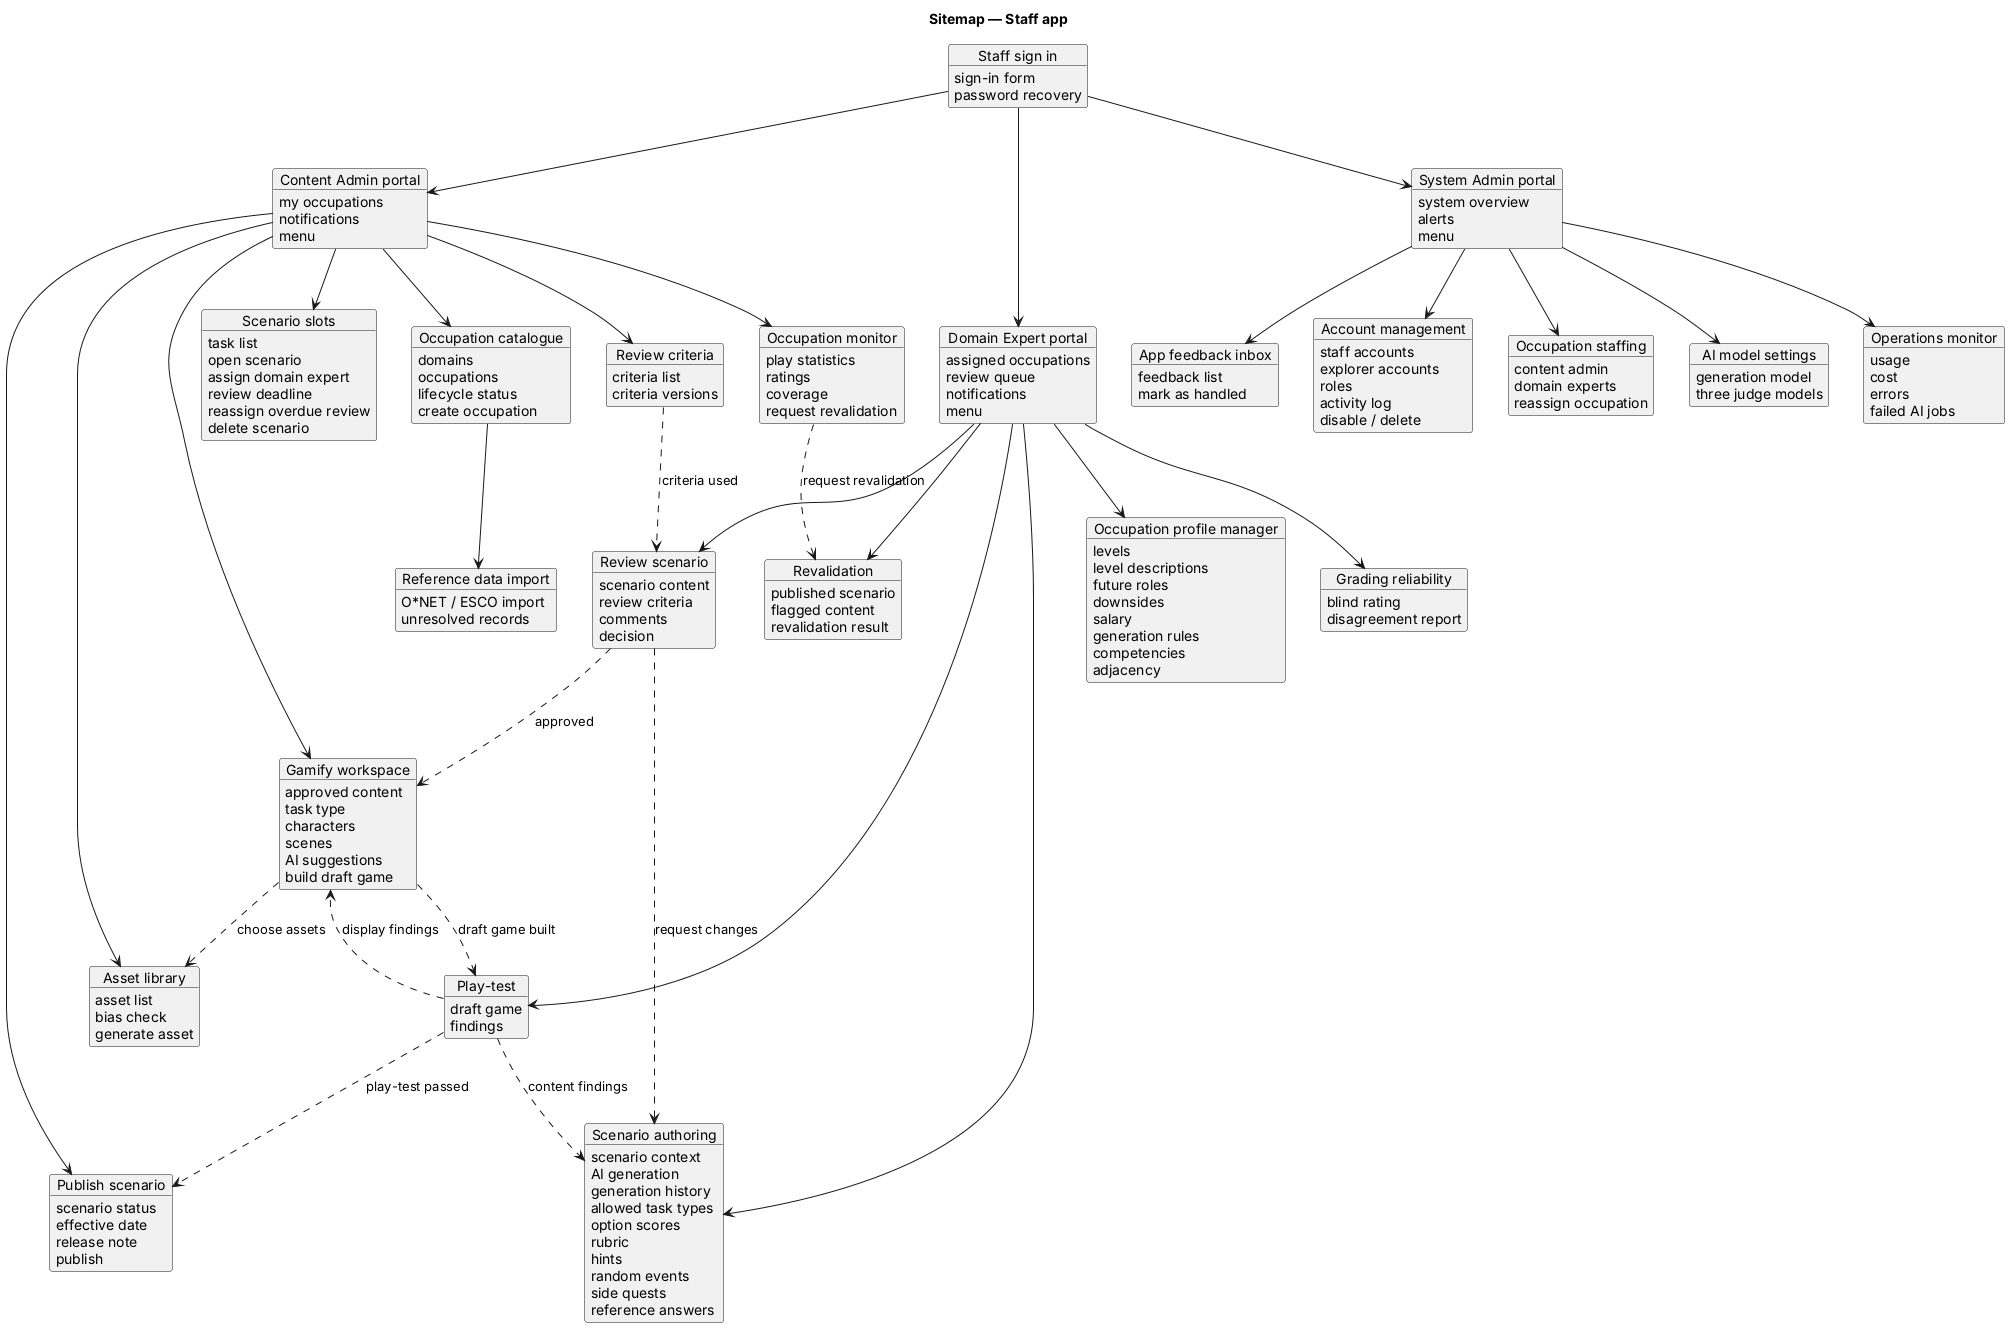
\includegraphics[width=\linewidth,keepaspectratio]{figures/SITE-02_StaffApp.png}
\caption{Sitemap of the staff application (SITE-02)}
\end{figure}
\end{landscape}
